%package list
\documentclass{article}
\usepackage[top=3cm, bottom=3cm, outer=3cm, inner=3cm]{geometry}
\usepackage{multicol}
\usepackage{graphicx}
\usepackage{url}
%\usepackage{cite}
\usepackage{hyperref}
\usepackage{array}
%\usepackage{multicol}
\newcolumntype{x}[1]{>{\centering\arraybackslash\hspace{0pt}}p{#1}}
\usepackage{natbib}
\usepackage{pdfpages}
\usepackage{multirow}
\usepackage[normalem]{ulem}
\useunder{\uline}{\ul}{}
\usepackage{svg}
\usepackage{xcolor}
\usepackage{listings}
\lstdefinestyle{ascii-tree}{
    literate={├}{|}1 {─}{--}1 {└}{+}1 
  }
\lstset{basicstyle=\ttfamily,
  showstringspaces=false,
  commentstyle=\color{red},
  keywordstyle=\color{blue}
}
%\usepackage{booktabs}
\usepackage{caption}
\usepackage{subcaption}
\usepackage{float}
\usepackage{array}

\newcolumntype{M}[1]{>{\centering\arraybackslash}m{#1}}
\newcolumntype{N}{@{}m{0pt}@{}}


%%%%%%%%%%%%%%%%%%%%%%%%%%%%%%%%%%%%%%%%%%%%%%%%%%%%%%%%%%%%%%%%%%%%%%%%%%%%
%%%%%%%%%%%%%%%%%%%%%%%%%%%%%%%%%%%%%%%%%%%%%%%%%%%%%%%%%%%%%%%%%%%%%%%%%%%%
\newcommand{\itemStudent}{Arles Carrasco Choque, Jean Carlo Chara Condori, Reyser Zapata Butron, Daniela Choquecondo Aspilcueta}
\newcommand{\itemCourse}{Pweb2-Lab}
\newcommand{\itemSemester}{III}
\newcommand{\itemUniversity}{Universidad Nacional de San Agustín de Arequipa}
\newcommand{\itemFaculty}{Facultad de Ingeniería de Producción y Servicios}
\newcommand{\itemDepartment}{Departamento Académico de Ingeniería de Sistemas e Informática}
\newcommand{\itemSchool}{Escuela Profesional de Ingeniería de Sistemas}
\newcommand{\itemAcademic}{2023 - A}
\newcommand{\itemInput}{Del 5 Junio 2023}
\newcommand{\itemOutput}{Al 20 Junio 2023}
\newcommand{\itemPracticeNumber}{05}
\newcommand{\itemTheme}{Django}
%%%%%%%%%%%%%%%%%%%%%%%%%%%%%%%%%%%%%%%%%%%%%%%%%%%%%%%%%%%%%%%%%%%%%%%%%%%%
%%%%%%%%%%%%%%%%%%%%%%%%%%%%%%%%%%%%%%%%%%%%%%%%%%%%%%%%%%%%%%%%%%%%%%%%%%%%

\usepackage[english,spanish]{babel}
\usepackage[utf8]{inputenc}
\AtBeginDocument{\selectlanguage{spanish}}
\renewcommand{\figurename}{Figura}
\renewcommand{\refname}{Referencias}
\renewcommand{\tablename}{Tabla} %esto no funciona cuando se usa babel
\AtBeginDocument{%
	\renewcommand\tablename{Tabla}
}

\usepackage{fancyhdr}
\pagestyle{fancy}
\fancyhf{}
\setlength{\headheight}{30pt}
\renewcommand{\headrulewidth}{1pt}
\renewcommand{\footrulewidth}{1pt}
\fancyhead[L]{\raisebox{-0.2\height}{
\includegraphics[width=3cm]{img/logo_episunsa.png}}}
\fancyhead[C]{\fontsize{7}{7}\selectfont	\itemUniversity \\ \itemFaculty \\ \itemDepartment \\ \itemSchool \\ \textbf{\itemCourse}}
\fancyhead[R]{\raisebox{-0.2\height}{
\includegraphics[width=1.2cm]{img/logo_abet}}}
\fancyfoot[L]{Estudiante Juan Perez Perez}
\fancyfoot[C]{\itemCourse}
\fancyfoot[R]{Página \thepage}

% para el codigo fuente
\usepackage{listings}
\usepackage{color, colortbl}
\definecolor{dkgreen}{rgb}{0,0.6,0}
\definecolor{gray}{rgb}{0.5,0.5,0.5}
\definecolor{mauve}{rgb}{0.58,0,0.82}
\definecolor{codebackground}{rgb}{0.95, 0.95, 0.92}
\definecolor{tablebackground}{rgb}{0.8, 0, 0}

\lstset{frame=tb,
	language=bash,
	aboveskip=3mm,
	belowskip=3mm,
	showstringspaces=false,
	columns=flexible,
	basicstyle={\small\ttfamily},
	numbers=none,
	numberstyle=\tiny\color{gray},
	keywordstyle=\color{blue},
	commentstyle=\color{dkgreen},
	stringstyle=\color{mauve},
	breaklines=true,
	breakatwhitespace=true,
	tabsize=3,
	backgroundcolor= \color{codebackground},
}

\begin{document}
	
	\vspace*{10px}
	
	\begin{center}	
		\fontsize{17}{17} \textbf{ Informe de Laboratorio \itemPracticeNumber}
	\end{center}
	\centerline{\textbf{\Large Tema: \itemTheme}}
	%\vspace*{0.5cm}	

	\begin{flushright}
		\begin{tabular}{|M{2.5cm}|N|}
			\hline 
			\rowcolor{tablebackground}
			\color{white} \textbf{Nota}  \\
			\hline 
			     \\[30pt]
			\hline 			
		\end{tabular}
	\end{flushright}	

	\begin{table}[H]
		\begin{tabular}{|x{4.7cm}|x{4.8cm}|x{4.8cm}|}
			\hline 
			\rowcolor{tablebackground}
			\color{white} \textbf{Estudiante} & \color{white}\textbf{Escuela}  & \color{white}\textbf{Asignatura}   \\
			\hline 
			{\itemStudent \par \itemEmail} & \itemSchool & {\itemCourse \par Semestre: III}     \\
			\hline 			
		\end{tabular}
	\end{table}		
	
	\begin{table}[H]
		\begin{tabular}{|x{4.7cm}|x{4.8cm}|x{4.8cm}|}
			\hline 
			\rowcolor{tablebackground}
			\color{white}\textbf{Laboratorio} & \color{white}\textbf{Tema}  & \color{white}\textbf{Duración}   \\
			\hline 
			\itemPracticeNumber & \itemTheme & 04 horas   \\
			\hline 
		\end{tabular}
	\end{table}
	
	\begin{table}[H]
		\begin{tabular}{|x{4.7cm}|x{4.8cm}|x{4.8cm}|}
			\hline 
			\rowcolor{tablebackground}
			\color{white}\textbf{Semestre académico} & \color{white}\textbf{Fecha de inicio}  & \color{white}\textbf{Fecha de entrega}   \\
			\hline 
			\itemAcademic & \itemInput &  \itemOutput  \\
			\hline 
		\end{tabular}
	\end{table}
	\section{Competencias del Curso}
	\begin{itemize}		
 \item General: C.c. Diseña responsablemente aplicaciones web, sus componentes o procesos para satisfacer necesidades dentro de restricciones realistas: económicas, medio ambientales, sociales, políticas, éticas, de salud, de seguridad, manufacturación y sostenibilidad.

\item Específica: C.m. Construye responsablemente soluciones con tecnología web siguiendo un proceso adecuado llevando a cabo las pruebas ajustada a los recursos disponibles del cliente.

 \item Específica: C.p. Aplica de forma flexible t ́ecnicas, métodos, principios, normas, estándares y herramientas del desarrollo web necesarias para la construcci ́on de aplicaciones web e implementación de estos sistemas en una organización.

	\end{itemize}		
 
	\section{Resultados del Estudiante}
	\begin{itemize}		
 \item RE. 2 La capacidad de aplicar dise ̃no de ingenier ́ıa para producir soluciones a problemas y diseñar sistemas, componentes o procesos para satisfacer necesidades específicas dentro de consideraciones realistas en los aspectos de salud p ́ublica, seguridad y bienestar; factores globales, culturales, sociales, económicos y ambientales.

\item RE. 8 La capacidad de crear, seleccionar y utilizar técnicas, habilidades, recursos y herramientas modernas de ingeniería y tecnologías de la información, incluyendo la predicción y el modelamiento, con una comprensión de las limitaciones.
	\end{itemize}


  	\section{Tarea}
	\begin{itemize}		
Elabore un primer informe grupal de la aplicación que desarrollará durante este semestre. Utilicen todas las recomendaciones dadas en la aplicación library.
Acuerdos :
\item Los grupos pueden estar conformado por 1 a 4 integrantes.
\item Solo se presenta un informe grupal.
\item Solo se revisa un repositorio. (El único que esté en el informe grupal).
\item Todos los integrantes del grupo tienen una copia del laboratorio e informe en su repositorio privado.
\item Todos los integrantes deben pertenecer al mismo grupo de laboratorio.
\item El docente preguntar ́a en cualquier momento a un integrante sobre el proyecto, codigo fuente, avance.

	\end{itemize}
		
	\section{Resolución}
	\begin{itemize}
 \item El laboratorio se organizó de la siguiente manera: 
  \item Ingresamos a nuestra carpeta "almacen" y tenemos el archivo "settings.py".
	\begin{figure}[H]
		\centering
		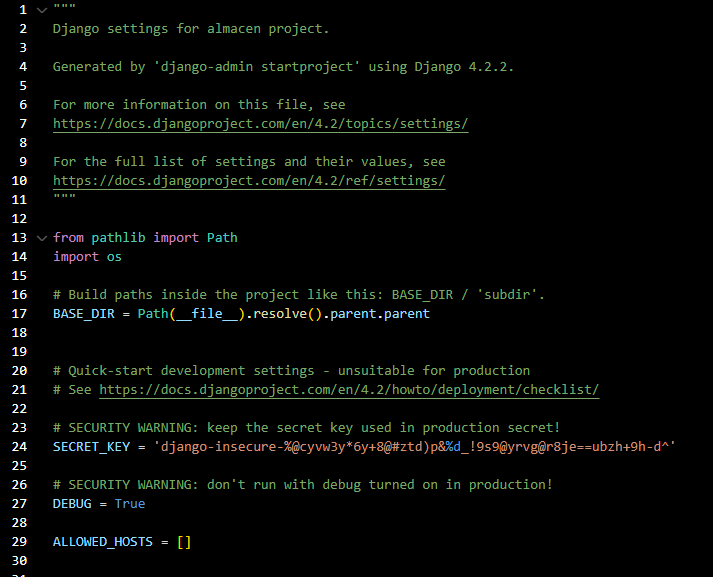
\includegraphics[width=0.8\textwidth,keepaspectratio]{Latex/img/settings1.png}
		%\includesvg{img/automata.svg}
		%\label{img:mot2}
		%\caption{Product backlog.}
	\end{figure}
	\end{itemize}
 \begin{itemize}
 \item Este código establece la configuración inicial de un proyecto Django. Se define la ruta principal del proyecto.
	\begin{figure}[H]
		\centering
		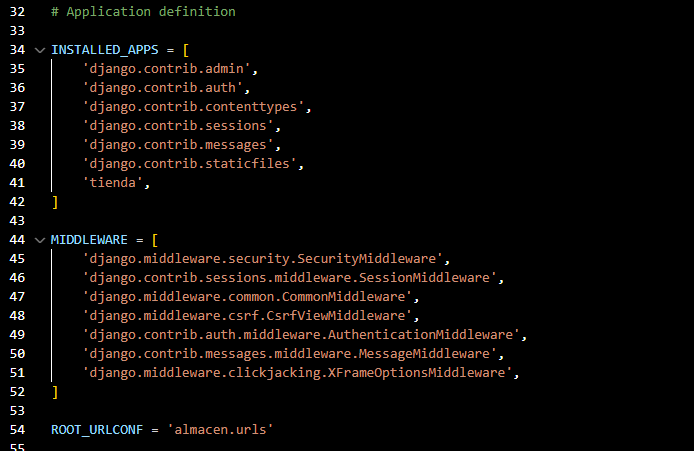
\includegraphics[width=0.8\textwidth,keepaspectratio]{Latex/img/settings2.png}
		%\includesvg{img/automata.svg}
		%\label{img:mot2}
		%\caption{Product backlog.}
	\end{figure}
	\end{itemize}
 \begin{itemize}
 \item Se configura las aplicaciones y el middleware en el proyecto. Se definen tres variables:
 \item "INSTALLED-APPS" ,"MIDDLEWARE" y "ROOT-URLCONF".
	\begin{figure}[H]
		\centering
		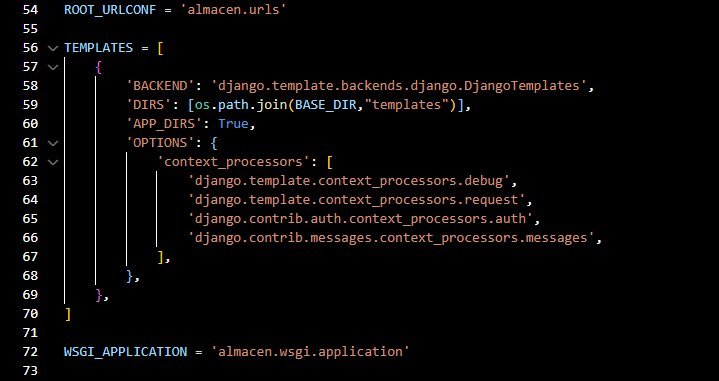
\includegraphics[width=0.8\textwidth,keepaspectratio]{Latex/img/settings3.png}
		%\includesvg{img/automata.svg}
		%\label{img:mot2}
		%\caption{Product backlog.}
	\end{figure}
	\end{itemize}

\begin{itemize}
 \item En este código, se están configurando aspectos clave en Django:
  \item ROOT-URLCONF: Se define el archivo de configuración de URL de la aplicación como 'almacen.urls'.
  \item TEMPLATES: Se establecen las configuraciones de las plantillas de Django, indicando las ubicaciones de los directorios de plantillas y agregando procesadores de contexto adicionales.
  \item WSGI-APPLICATION: Se asigna el módulo 'almacen.wsgi.application' como la aplicación WSGI para servir la aplicación Django.
	\begin{figure}[H]
		\centering
		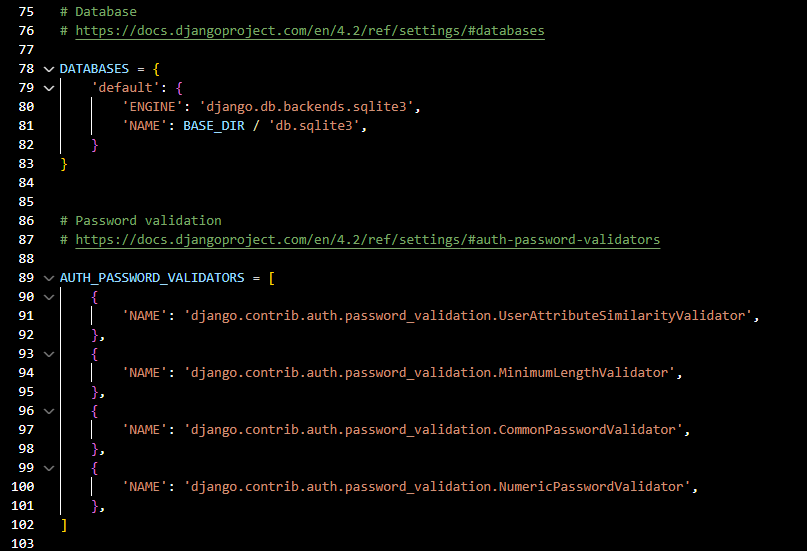
\includegraphics[width=0.8\textwidth,keepaspectratio]{Latex/img/settings4.png}
		%\includesvg{img/automata.svg}
		%\label{img:mot2}
		%\caption{Product backlog.}
	\end{figure}
	\end{itemize}

 
\begin{itemize}
Se realiza la configuración de la base de datos y las validaciones de contraseñas en Django. Son esenciales para asegurar el correcto funcionamiento y la seguridad de la aplicación Django, al definir la base de datos utilizada y las reglas de validación para las contraseñas de los usuarios.
  \item DATABASES: Se establece la configuración de la base de datos, utilizando SQLite como motor y especificando el nombre y ubicación del archivo de la base de datos.
  \item AUTH-PASSWORD-VALIDATORS: Se definen las validaciones de contraseñas para la autenticación de usuarios. Cada validación verifica diferentes aspectos, como la similitud con atributos del usuario, la longitud mínima, la utilización de contraseñas comunes y la inclusión de al menos un número.

	\begin{figure}[H]
		\centering
		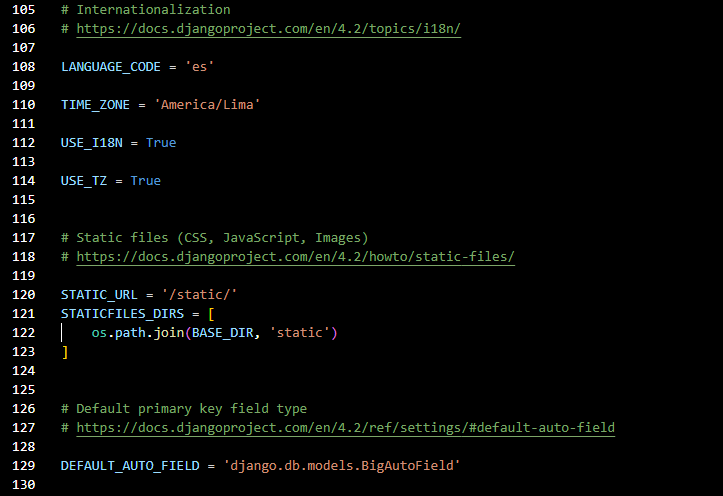
\includegraphics[width=0.8\textwidth,keepaspectratio]{Latex/img/settings5.png}
		%\includesvg{img/automata.svg}
		%\label{img:mot2}
		%\caption{Product backlog.}
	\end{figure}
	\end{itemize}
 \begin{itemize}
		\item En el archivo "urls.py", se definen las rutas y a que función apuntan, estas funciones se encuentran en nuestro archivo "views.py", donde nos muestra las vistas y lo que se va a visualizar.
	\begin{figure}[H]
		\centering
		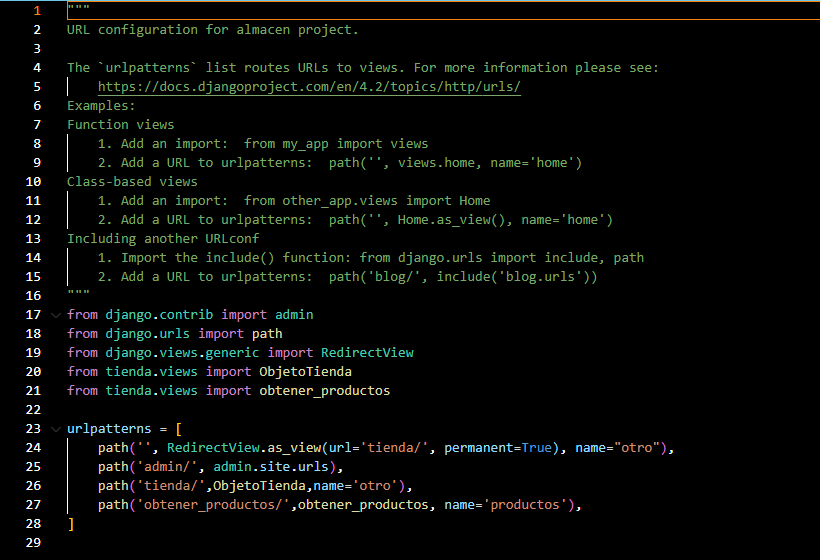
\includegraphics[width=0.8\textwidth,keepaspectratio]{Latex/img/urls.png}
		%\includesvg{img/automata.svg}
		%\label{img:mot2}
		%\caption{Product backlog.}
	\end{figure}
	\end{itemize}
  \begin{itemize}
		\item Entonces se configura las URLs de la aplicación Django, definiendo las rutas y asociando las vistas correspondientes a cada URL. 
	\begin{figure}[H]
		\centering
		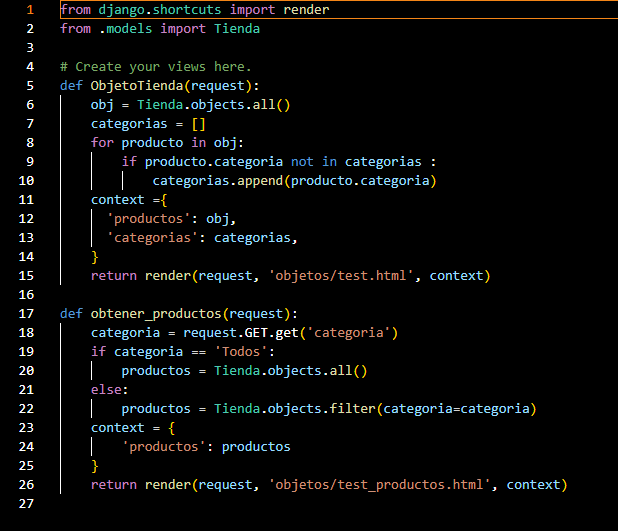
\includegraphics[width=0.8\textwidth,keepaspectratio]{Latex/img/views.png}
		%\includesvg{img/automata.svg}
		%\label{img:mot2}
		%\caption{Product backlog.}
	\end{figure}
	\end{itemize}
 \begin{itemize}
		\item  Estas vistas se encargan de procesar las solicitudes HTTP y devolver las respuestas correspondientes, utilizando los modelos y las plantillas (se recibe un parámetro "categoria" de la solicitud GET, obtiene los productos correspondientes a esa categoría y los pasa a una plantilla para su renderizado). 
	\begin{figure}[H]
		\centering
		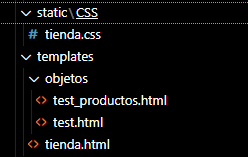
\includegraphics[width=0.8\textwidth,keepaspectratio]{Latex/img/css-templates.png}
		%\includesvg{img/automata.svg}
		%\label{img:mot2}
		%\caption{Product backlog.}
	\end{figure}
	\end{itemize}
 \begin{itemize}
		\item   En nuestra carpeta "static" guardamos el archivo css que le dará el diseño a nuestra página, por otro lado también en la carpeta "templates" se encuentra la estructura de la página principal, las plantillas que serán visualizadas por el usuario final. 
	\begin{figure}[H]
		\centering
		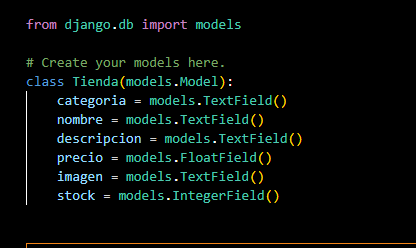
\includegraphics[width=0.8\textwidth,keepaspectratio]{Latex/img/models.png}
		%\includesvg{img/automata.svg}
		%\label{img:mot2}
		%\caption{Product backlog.}
	\end{figure}
	\end{itemize}
  \begin{itemize}
		\item    En el archivo "models.py" , se define el modelo de datos "Tienda" en Django, que representa una tabla en la base de datos con campos como categoría, nombre, descripción, precio, imagen y stock. Permite interactuar con los datos de la tienda mediante operaciones CRUD utilizando Django ORM.

\section{Visualización de la Página:}
	\begin{figure}[H]
		\centering
		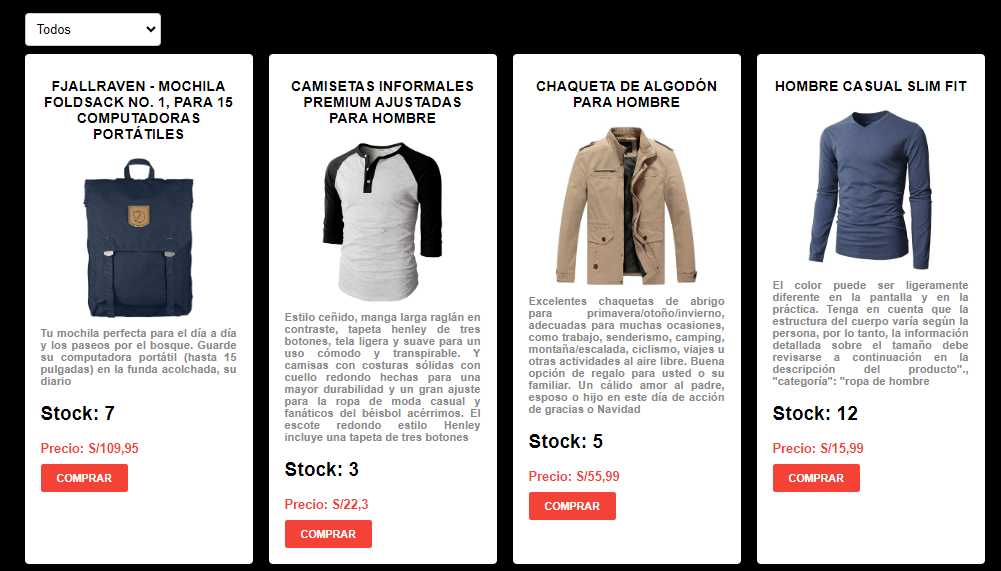
\includegraphics[width=0.8\textwidth,keepaspectratio]{Latex/img/todo.png}
		%\includesvg{img/automata.svg}
		%\label{img:mot2}
		%\caption{Product backlog.}
	\end{figure}
\begin{figure}[H]
		\centering
		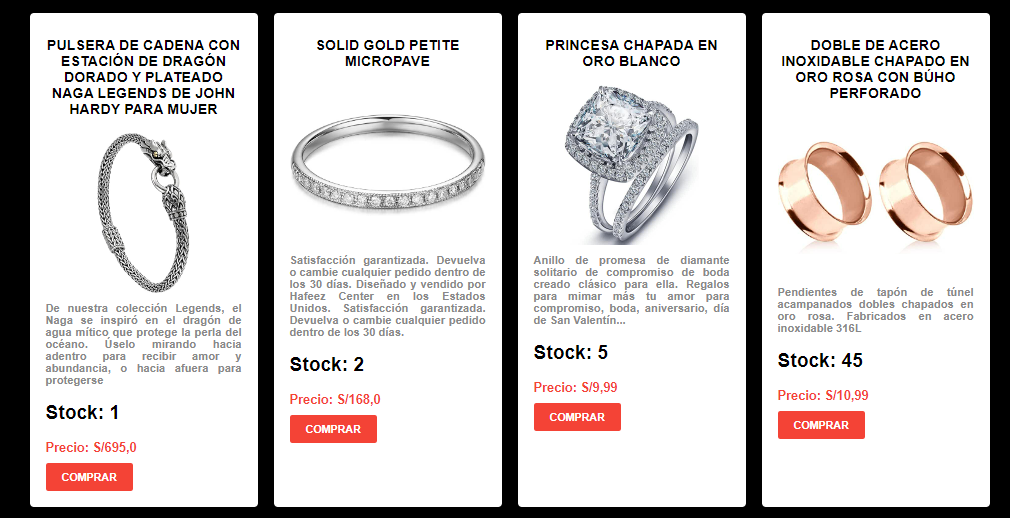
\includegraphics[width=0.8\textwidth,keepaspectratio]{Latex/img/todo2.png}
		%\includesvg{img/automata.svg}
		%\label{img:mot2}
		%\caption{Product backlog.}
	\end{figure}
 \item  \begin{figure}[H]
		\centering
		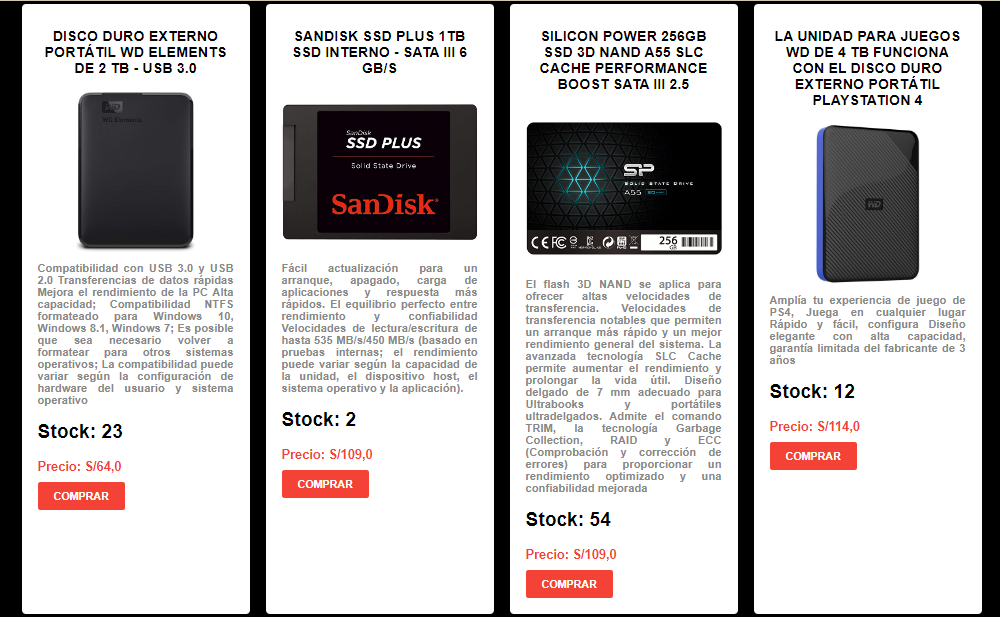
\includegraphics[width=0.8\textwidth,keepaspectratio]{Latex/img/todo3.png}
		%\includesvg{img/automata.svg}
		%\label{img:mot2}
		%\caption{Product backlog.}
	\end{figure}
\item Por partes - Electrónica:
\begin{figure}[H]
		\centering
		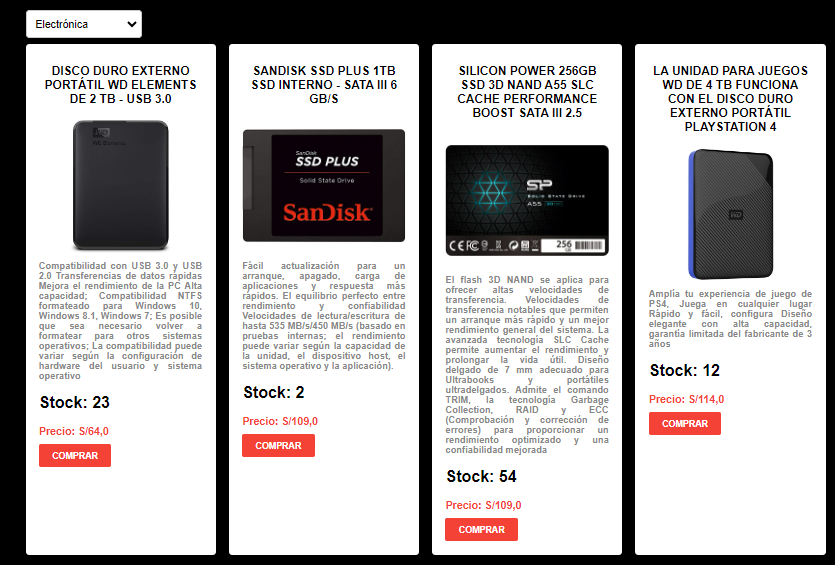
\includegraphics[width=0.8\textwidth,keepaspectratio]{Latex/img/electronica.png}
		%\includesvg{img/automata.svg}
		%\label{img:mot2}
		%\caption{Product backlog.}
	\end{figure}

\item Por partes - Joyería:
\begin{figure}[H]
		\centering
		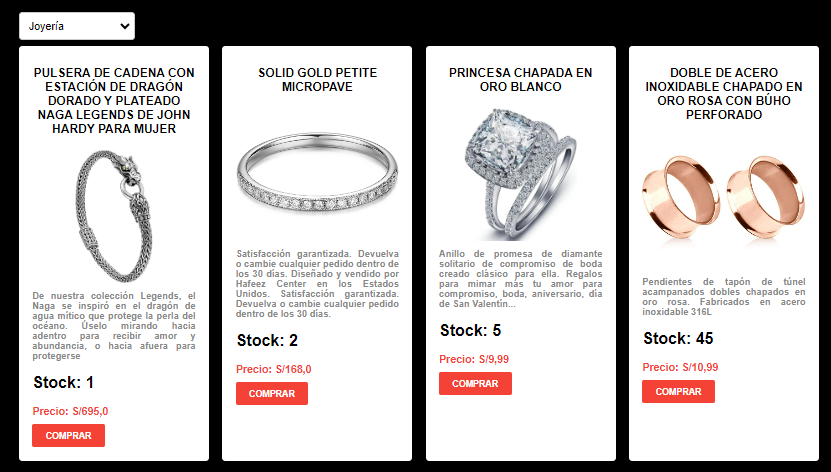
\includegraphics[width=0.8\textwidth,keepaspectratio]{Latex/img/joyeria.png}
		%\includesvg{img/automata.svg}
		%\label{img:mot2}
		%\caption{Product backlog.}
	\end{figure}

\item Por partes - Ropa de Hombre:
\begin{figure}[H]
		\centering
		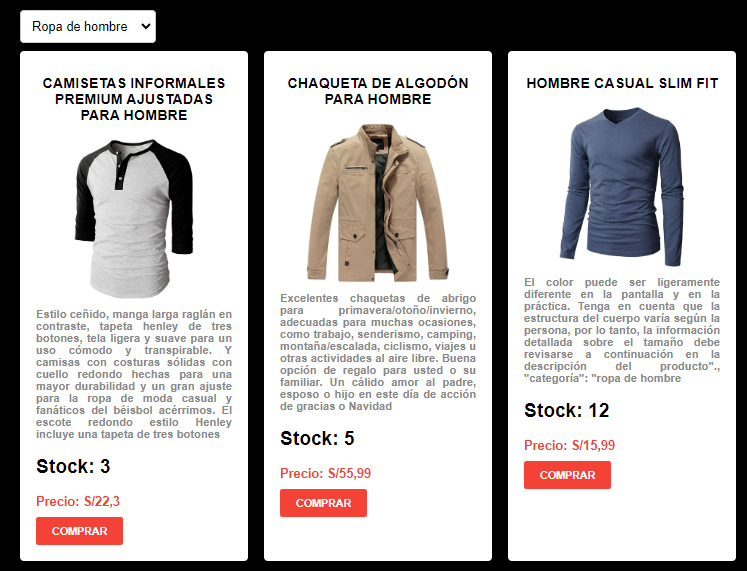
\includegraphics[width=0.8\textwidth,keepaspectratio]{Latex/img/ropahombre.png}
		%\includesvg{img/automata.svg}
		%\label{img:mot2}
		%\caption{Product backlog.}
	\end{figure}


\section{Referencias}
\begin{itemize}			
	\item \url{https://developer.mozilla.org/en-US/docs/Learn/Server-side/Django/Tutorial_local_
library_website}
\end{itemize}	
	
 \item 
	\section{Preguntas}
	\begin{itemize}
 \item Arles Carrasco: "Al estudiar Django, aprendí a aprovechar la estructura de directorios y archivos predefinidos que proporciona el framework, tambien facilita la navegación y el mantenimiento del código. Siguiendo esta estructura y utilizando los nombres de archivos y directorios recomendados, se mejora la legibilidad y la colaboración en el desarrollo de proyectos Django. Tambien al usar los componentes que ya tiene integrado se acelera el proceso de crear una pagina web como el administrador el cual puede agregar de una manera mas facil los objetos, tambien usuarios y rellenar formularios".

\item Jean Carlo Chara: " He aprendido a crear proyectos de Django, los cuales actuaron como contenedores para mis aplicaciones facilitando la organizacion de mi codigo. Asimismo he aprendido a crear modelos, los cuales me fueron de apoyo para la gestion de atributos gracias a la base de datos de Django. Aprendí a crear url's con path, sincronizar los modelos con los templates con la ayuda de etiquetas {{}}, accediendo a los modelos almacenados en la base de datos y renderizandolos. Finalmente he aprendido a realizar una pequeña conexión con la base de datos de Django utilizando AJAX realizando una peticion para devolver los datos de un modelo. "

 \item Reyser Zapata: " Pude profundizar mis conocimientos en el manejo de vistas, lo que me ha permitido implementar lógica de negocio personalizada y manipular datos de manera efectiva. Además, he dominado el uso de plantillas, lo que me ha brindado la capacidad de crear interfaces de usuario dinámicas y atractivas, conectando de manera fluida las vistas con el contenido visual. Por otro lado pude aprender sobre plantillas, formularios y enrutamiento de URL. Estas habilidades me permiten desarrollar aplicaciones web robustas, interactivas y seguras, brindando una experiencia atractiva a los usuarios finales. Estoy emocionado de seguir ampliando mis conocimientos en Django y aplicarlos en futuros proyectos. "
 \item Daniela Choquecondo: "Aprendí a aprovechar su estructura de directorios y archivos predefinidos, lo que facilitó la navegación y el mantenimiento de mi código. Seguí esta estructura y utilicé los nombres recomendados para mejorar la legibilidad y colaboración en el desarrollo de mis proyectos. También utilicé los componentes integrados en Django, como el administrador, para acelerar la creación de páginas web y simplificar la gestión de objetos, usuarios y formularios. Adquirí habilidades para crear proyectos Django, organizar mi código en aplicaciones y trabajar con modelos para gestionar los atributos en la base de datos. Aprendí a crear URLs con path, sincronizar modelos con plantillas utilizando etiquetas y renderizar datos almacenados en la base de datos. Además, exploré la conexión con la base de datos mediante AJAX para obtener datos de manera eficiente."

	\end{itemize}
 
	\section{URL de Repositorio Github}
	\begin{itemize}
 \item Repositorio del Grupo - Lab05 (Django):    
\url{https://github.com/carrascoArles/ProyectoPweb2.git}
	\end{itemize}

\section{Referencias}
\begin{itemize}			
	\item \url{https://docs.oracle.com/javase/7/docs/api/java/util/List.html}
	\item \url{https://docs.oracle.com/javase/tutorial/java/generics/types.html}
\end{itemize}	
	
%\clearpage
%\bibliographystyle{apalike}
%\bibliographystyle{IEEEtranN}
%\bibliography{bibliography}
			
\end{document}